\documentclass[tikz,border=4pt]{standalone}
\usepackage{amsmath}
\usepackage{sansmath}
\usetikzlibrary{arrows.meta,calc,decorations.pathmorphing,positioning}

\definecolor{ink}{HTML}{24303A}
\definecolor{muted}{HTML}{64727D}
\definecolor{sulfur}{HTML}{D89B16}
\definecolor{sulfurLight}{HTML}{F8E7B2}
\definecolor{polymer}{HTML}{367C91}
\definecolor{polymerLight}{HTML}{D9EDF1}
\definecolor{trap}{HTML}{B64A5A}
\definecolor{trapLight}{HTML}{F5DDE1}
\definecolor{field}{HTML}{6755A5}
\definecolor{fieldLight}{HTML}{E8E2F5}
\definecolor{panel}{HTML}{F8FAFB}
\definecolor{linegray}{HTML}{CCD5DA}

\tikzset{
  every node/.style={font=\sffamily, text=ink},
  panelbox/.style={draw=linegray, fill=panel, rounded corners=2.2pt, line width=.7pt},
  panelletter/.style={circle, fill=ink, text=white, font=\sffamily\bfseries\small,
    inner sep=0pt, minimum size=5.6mm},
  paneltitle/.style={font=\sffamily\bfseries\small, anchor=west},
  label/.style={font=\sffamily\scriptsize, text=muted},
  tinylabel/.style={font=\sffamily\tiny, text=muted},
  bond/.style={line width=1.15pt, draw=ink},
  sulfurbond/.style={line width=1.4pt, draw=sulfur},
  apparatus/.style={draw=ink, fill=white, rounded corners=1pt, line width=.7pt},
  axis/.style={-{Stealth[length=2.2mm]}, draw=muted, line width=.55pt},
  data/.style={draw=polymer, line width=1.35pt},
  derived/.style={draw=trap, line width=1.35pt},
  flow/.style={-{Stealth[length=2.4mm]}, draw=muted, line width=.8pt},
}

\begin{document}
\sansmath
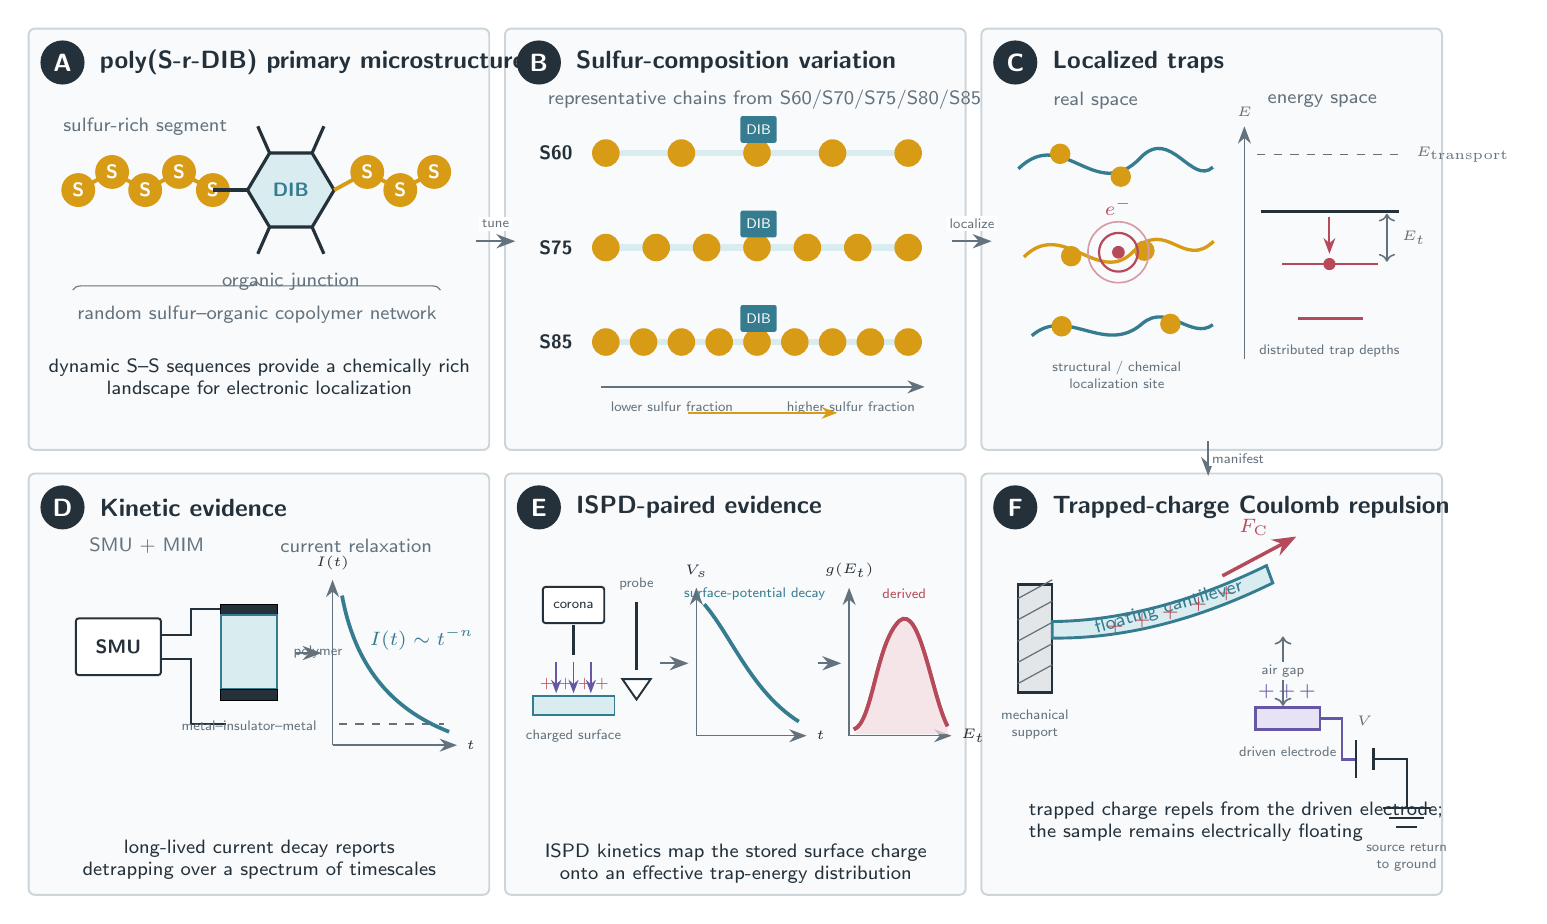
\begin{tikzpicture}[x=1cm,y=1cm]

% panel frames
\foreach \x/\y/\w/\h in {0/7.45/5.85/5.35,6.05/7.45/5.85/5.35,12.10/7.45/5.85/5.35,
                            0/1.80/5.85/5.35,6.05/1.80/5.85/5.35,12.10/1.80/5.85/5.35}
  \path[panelbox] (\x,\y) rectangle ++(\w,\h);

% ------------------------------------------------------------------ A
\node[panelletter] at (.43,12.37) {A};
\node[paneltitle] at (.78,12.37) {poly(S-r-DIB) primary microstructure};

\begin{scope}[shift={(.48,9.70)}]
  % sulfur-rich backbone
  \draw[sulfurbond] (.15,1.05) -- (.58,1.28) -- (1.00,1.05) -- (1.43,1.28) -- (1.86,1.05);
  \foreach \x in {.15,.58,1.00,1.43,1.86}
    \node[circle,fill=sulfur,text=white,font=\sffamily\bfseries\scriptsize,
      minimum size=4.3mm,inner sep=0pt] at (\x,{1.05+0.23*mod(round((\x-.15)/.425),2)}) {S};
  \node[label,anchor=south] at (1.0,1.62) {sulfur-rich segment};
  % organic DIB junction
  \draw[bond] (1.86,1.05) -- (2.30,1.05);
  \draw[bond,fill=polymerLight] (2.30,1.05) -- (2.58,1.52) -- (3.12,1.52) --
    (3.40,1.05) -- (3.12,.58) -- (2.58,.58) -- cycle;
  \draw[bond] (2.58,1.52) -- (2.43,1.86);
  \draw[bond] (3.12,1.52) -- (3.27,1.86);
  \draw[bond] (2.58,.58) -- (2.43,.24);
  \draw[bond] (3.12,.58) -- (3.27,.24);
  \node[font=\sffamily\bfseries\scriptsize,text=polymer] at (2.85,1.05) {DIB};
  \node[label,anchor=north] at (2.85,.12) {organic junction};
  % continuing sulfur chain
  \draw[sulfurbond] (3.40,1.05) -- (3.82,1.28) -- (4.24,1.05) -- (4.67,1.28);
  \foreach \x/\yy in {3.82/1.28,4.24/1.05,4.67/1.28}
    \node[circle,fill=sulfur,text=white,font=\sffamily\bfseries\scriptsize,
      minimum size=4.3mm,inner sep=0pt] at (\x,\yy) {S};
  \draw[decorate,decoration={brace,amplitude=3pt},draw=muted] (.08,-.22) -- (4.75,-.22);
  \node[label,anchor=north] at (2.42,-.30) {random sulfur--organic copolymer network};
\end{scope}
\node[font=\sffamily\scriptsize,align=center,text=ink] at (2.93,8.35)
  {dynamic S--S sequences provide a chemically rich\\landscape for electronic localization};

% ------------------------------------------------------------------ B
\node[panelletter] at (6.48,12.37) {B};
\node[paneltitle] at (6.83,12.37) {Sulfur-composition variation};
\node[label,anchor=west] at (6.47,11.90) {representative chains from S60/S70/S75/S80/S85};

\begin{scope}[shift={(6.55,8.10)}]
  \foreach \yy/\name/\count in {3.12/S60/5,1.92/S75/7,.72/S85/9}{
    \node[font=\sffamily\bfseries\scriptsize,anchor=east,text=ink] at (.48,\yy) {\name};
    \draw[line width=2.4pt,polymerLight,rounded corners] (.72,\yy) -- (4.70,\yy);
    \foreach \i in {1,...,\count}{
      \pgfmathsetmacro{\xx}{.78+(\i-1)*(3.84/(\count-1))}
      \node[circle,fill=sulfur,minimum size=3.5mm,inner sep=0pt] at (\xx,\yy) {};
    }
    \node[rectangle,rounded corners=.8pt,fill=polymer,text=white,font=\sffamily\tiny,
      minimum width=4.6mm,minimum height=3.4mm,inner sep=0pt] at (2.72,{\yy+.30}) {DIB};
  }
  \draw[axis] (.72,.15) -- (4.83,.15);
  \node[tinylabel,anchor=north west] at (.72,.08) {lower sulfur fraction};
  \node[tinylabel,anchor=north east] at (4.83,.08) {higher sulfur fraction};
  \draw[-{Stealth[length=2mm]},line width=.7pt,sulfur] (1.82,-.18) -- (3.72,-.18);
\end{scope}

% ------------------------------------------------------------------ C
\node[panelletter] at (12.53,12.37) {C};
\node[paneltitle] at (12.88,12.37) {Localized traps};
\node[label] at (13.55,11.88) {real space};
\node[label] at (16.43,11.88) {energy space};

\begin{scope}[shift={(12.42,8.18)}]
  % disordered real-space network
  \draw[polymer,line width=1.2pt] (.15,2.84) .. controls (.72,3.40) and (1.13,2.38) .. (1.70,2.98)
    .. controls (2.08,3.38) and (2.35,2.62) .. (2.62,2.86);
  \draw[sulfur,line width=1.2pt] (.22,1.72) .. controls (.72,2.22) and (1.18,1.32) .. (1.62,1.80)
    .. controls (2.03,2.22) and (2.25,1.55) .. (2.63,1.92);
  \draw[polymer,line width=1.2pt] (.32,.72) .. controls (.77,1.11) and (1.25,.45) .. (1.73,.88)
    .. controls (2.05,1.14) and (2.35,.66) .. (2.62,.86);
  \foreach \x/\y in {.68/3.03,1.45/2.74,.82/1.73,1.75/1.80,.70/.84,2.08/.87}
    \node[circle,fill=sulfur,minimum size=2.6mm,inner sep=0pt] at (\x,\y) {};
  \fill[trap] (1.42,1.78) circle (2.3pt);
  \draw[trap,line width=.8pt] (1.42,1.78) circle (7pt);
  \draw[trap!55,line width=.6pt] (1.42,1.78) circle (11pt);
  \node[font=\sffamily\bfseries\scriptsize,text=trap,anchor=south] at (1.42,2.12) {$e^{-}$};
  \node[tinylabel,align=center] at (1.40,.22) {structural / chemical\\localization site};
  % energy landscape
  \draw[axis] (3.02,.42) -- (3.02,3.38) node[above,font=\sffamily\tiny,text=muted] {$E$};
  \draw[muted,line width=.55pt,dashed] (3.18,3.02) -- (5.06,3.02);
  \node[tinylabel,anchor=west] at (5.08,3.02) {$E_\mathrm{transport}$};
  \draw[ink,line width=1pt] (3.23,2.30) -- (4.98,2.30);
  \draw[trap,line width=1pt] (3.50,1.63) -- (4.72,1.63);
  \draw[trap,line width=1pt] (3.70,.94) -- (4.52,.94);
  \fill[trap] (4.10,1.63) circle (2.2pt);
  \draw[-{Stealth[length=2mm]},trap,line width=.75pt] (4.10,2.23) -- (4.10,1.76);
  \draw[<->,muted,line width=.55pt] (4.83,1.66) -- (4.83,2.27);
  \node[tinylabel,anchor=west] at (4.90,1.96) {$E_t$};
  \node[tinylabel] at (4.10,.52) {distributed trap depths};
\end{scope}

% ------------------------------------------------------------------ D
\node[panelletter] at (.43,6.72) {D};
\node[paneltitle] at (.78,6.72) {Kinetic evidence};
\node[label] at (1.50,6.23) {SMU + MIM};
\node[label] at (4.16,6.23) {current relaxation};

\begin{scope}[shift={(.36,2.25)}]
  % SMU and MIM stack
  \node[apparatus,minimum width=1.08cm,minimum height=.72cm,font=\sffamily\bfseries\scriptsize] (smu) at (.78,2.70) {SMU};
  \draw[ink,line width=.75pt] (1.32,2.85) -- (1.70,2.85) -- (1.70,3.18) -- (2.15,3.18);
  \draw[ink,line width=.75pt] (1.32,2.55) -- (1.70,2.55) -- (1.70,1.72) -- (2.15,1.72);
  \draw[fill=ink] (2.08,3.10) rectangle (2.80,3.24);
  \draw[fill=polymerLight,draw=polymer,line width=.7pt] (2.08,2.16) rectangle (2.80,3.10);
  \draw[fill=ink] (2.08,2.02) rectangle (2.80,2.16);
  \node[tinylabel,anchor=west] at (2.88,2.63) {polymer};
  \node[tinylabel] at (2.44,1.70) {metal--insulator--metal};
  \draw[flow] (3.02,2.62) -- (3.36,2.62);
  % decay graph
  \draw[axis] (3.50,1.45) -- (5.08,1.45) node[right,font=\sffamily\tiny] {$t$};
  \draw[axis] (3.50,1.45) -- (3.50,3.55) node[above,font=\sffamily\tiny] {$I(t)$};
  \draw[data] (3.62,3.35) .. controls (3.78,2.48) and (4.22,1.92) .. (4.98,1.62);
  \node[font=\sffamily\bfseries\scriptsize,text=polymer,anchor=west] at (3.85,2.80) {$I(t)\sim t^{-n}$};
  \draw[dashed,muted,line width=.5pt] (3.58,1.72) -- (4.92,1.72);
\end{scope}
\node[font=\sffamily\scriptsize,align=center] at (2.93,2.25)
  {long-lived current decay reports\\detrapping over a spectrum of timescales};

% ------------------------------------------------------------------ E
\node[panelletter] at (6.48,6.72) {E};
\node[paneltitle] at (6.83,6.72) {ISPD-paired evidence};

\begin{scope}[shift={(6.30,2.20)}]
  % corona/probe apparatus
  \node[apparatus,minimum width=.78cm,minimum height=.46cm,font=\sffamily\tiny] at (.62,3.28) {corona};
  \draw[ink,line width=.8pt] (.62,3.02) -- (.62,2.65);
  \draw[-{Stealth[length=1.7mm]},field,line width=.65pt] (.40,2.56) -- (.40,2.16);
  \draw[-{Stealth[length=1.7mm]},field,line width=.65pt] (.62,2.56) -- (.62,2.16);
  \draw[-{Stealth[length=1.7mm]},field,line width=.65pt] (.84,2.56) -- (.84,2.16);
  \draw[fill=polymerLight,draw=polymer,line width=.7pt] (.10,1.88) rectangle (1.14,2.12);
  \foreach \x in {.28,.52,.76,.98} \node[font=\sffamily\bfseries\tiny,text=trap] at (\x,2.28) {$+$};
  \draw[ink,line width=.8pt] (1.42,3.32) -- (1.42,2.45);
  \draw[fill=white,draw=ink,line width=.7pt] (1.24,2.34) -- (1.60,2.34) -- (1.42,2.08) -- cycle;
  \node[tinylabel] at (1.42,3.55) {probe};
  \node[tinylabel] at (.62,1.62) {charged surface};
  \draw[flow] (1.72,2.54) -- (2.08,2.54);
  % Vs plot
  \draw[axis] (2.18,1.62) -- (3.58,1.62) node[right,font=\sffamily\tiny] {$t$};
  \draw[axis] (2.18,1.62) -- (2.18,3.50) node[above,font=\sffamily\tiny] {$V_s$};
  \draw[data] (2.28,3.29) .. controls (2.62,2.90) and (2.88,2.18) .. (3.48,1.80);
  \node[tinylabel,text=polymer] at (2.92,3.42) {surface-potential decay};
  \draw[flow] (3.72,2.54) -- (4.02,2.54);
  % trap distribution
  \draw[axis] (4.12,1.62) -- (5.42,1.62) node[right,font=\sffamily\tiny] {$E_t$};
  \draw[axis] (4.12,1.62) -- (4.12,3.50) node[above,font=\sffamily\tiny] {$g(E_t)$};
  \draw[derived] (4.18,1.70) .. controls (4.42,1.78) and (4.46,2.80) .. (4.76,3.08)
    .. controls (5.02,3.30) and (5.17,2.12) .. (5.37,1.74);
  \fill[trapLight,opacity=.7] (4.18,1.64) .. controls (4.42,1.78) and (4.46,2.80) .. (4.76,3.08)
    .. controls (5.02,3.30) and (5.17,2.12) .. (5.37,1.74) -- (5.37,1.64) -- cycle;
  \draw[derived] (4.18,1.70) .. controls (4.42,1.78) and (4.46,2.80) .. (4.76,3.08)
    .. controls (5.02,3.30) and (5.17,2.12) .. (5.37,1.74);
  \node[tinylabel,text=trap] at (4.82,3.42) {derived};
\end{scope}
\node[font=\sffamily\scriptsize,align=center] at (8.98,2.20)
  {ISPD kinetics map the stored surface charge\\onto an effective trap-energy distribution};

% ------------------------------------------------------------------ F
\node[panelletter] at (12.53,6.72) {F};
\node[paneltitle] at (12.88,6.72) {Trapped-charge Coulomb repulsion};

\begin{scope}[shift={(12.38,2.10)}]
  % restrained mechanical support (no electrical connector)
  \draw[fill=muted!18,draw=ink,line width=.8pt] (.18,2.27) rectangle (.62,3.64);
  \foreach \yy in {2.38,2.65,2.92,3.19,3.46}
    \draw[muted,line width=.45pt] (.18,\yy) -- (.62,{\yy+.24});
  \node[tinylabel,align=center,anchor=north] at (.40,2.17) {mechanical\\support};
  % floating cantilever deflected away from electrode
  \draw[fill=polymerLight,draw=polymer,line width=1.05pt]
    (.62,3.17) .. controls (1.55,3.18) and (2.46,3.45) .. (3.34,3.88)
    -- (3.42,3.66) .. controls (2.48,3.20) and (1.55,2.95) .. (.62,2.96) -- cycle;
  \node[font=\sffamily\scriptsize,text=polymer,rotate=16] at (2.10,3.35) {floating cantilever};
  \foreach \x/\y in {1.42/3.10,1.76/3.18,2.12/3.28,2.48/3.39,2.83/3.53}
    \node[font=\sffamily\bfseries\scriptsize,text=trap] at (\x,\y) {$+$};
  \draw[-{Stealth[length=3mm]},trap,line width=1.25pt] (2.78,3.75) -- (3.72,4.25);
  \node[font=\sffamily\bfseries\scriptsize,text=trap,anchor=south] at (3.18,4.14) {$F_\mathrm{C}$};
  % air gap and driven electrode
  \draw[<->,muted,line width=.6pt] (3.55,2.98) -- (3.55,2.10);
  \node[tinylabel,fill=panel,inner sep=1pt] at (3.55,2.54) {air gap};
  \draw[fill=fieldLight,draw=field,line width=1.0pt] (3.20,1.80) rectangle (4.02,2.08);
  \foreach \x in {3.34,3.60,3.86}
    \node[font=\sffamily\bfseries\scriptsize,text=field] at (\x,2.28) {$+$};
  \node[tinylabel,anchor=north] at (3.61,1.70) {driven electrode};
  % compact voltage source and return ground
  \draw[field,line width=.85pt] (4.02,1.94) -- (4.30,1.94) -- (4.30,1.42) -- (4.48,1.42);
  \draw[ink,line width=.8pt] (4.48,1.18) -- (4.48,1.66);
  \draw[ink,line width=.8pt] (4.70,1.28) -- (4.70,1.56);
  \node[tinylabel,anchor=south] at (4.59,1.73) {$V$};
  \draw[ink,line width=.8pt] (4.70,1.42) -- (5.12,1.42) -- (5.12,.80);
  \draw[ink,line width=.8pt] (4.82,.80) -- (5.42,.80);
  \draw[ink,line width=.8pt] (4.90,.68) -- (5.34,.68);
  \draw[ink,line width=.8pt] (4.99,.56) -- (5.25,.56);
  \node[tinylabel,anchor=north,align=center] at (5.12,.47) {source return\\to ground};
  \node[font=\sffamily\scriptsize,align=left,anchor=west] at (.20,.63)
    {trapped charge repels from the driven electrode;\\the sample remains electrically floating};
\end{scope}

% cross-panel narrative
\draw[flow] (5.68,10.10) -- (6.18,10.10);
\draw[flow] (11.73,10.10) -- (12.23,10.10);
\draw[flow] (14.98,7.56) -- (14.98,7.12);
\node[tinylabel,fill=white,inner sep=1pt] at (5.93,10.32) {tune};
\node[tinylabel,fill=white,inner sep=1pt] at (11.98,10.32) {localize};
\node[tinylabel,fill=white,inner sep=1pt] at (15.36,7.34) {manifest};

\end{tikzpicture}
\end{document}
